\section{Double Integrals over General Regions} \label{S:11.3.Double_Integrals_General}

\vspace*{-14 pt}
\framebox{\hspace*{3 pt}
\parbox{6.25 in}{\begin{goals}
\item How do we define a double integral over a non-rectangular region?
\item What general form does an iterated integral over a non-rectangular region have?
\end{goals}} \hspace*{3 pt}}

\subsection*{Introduction}

Recall that we defined the double integral of a continuous function $f = f(x,y)$ over a rectangle $R = [a,b] \times [c,d]$ as
\[\iint_R f(x,y) \, dA = \lim_{m,n \to \infty} \sum_{j=1}^n \sum_{i=1}^m f(x_{ij}^*, y_{ij}^*) \cdot \Delta A,\]
where the notation is as described in Section~\ref{S:11.1.Double_Integrals_Rectangles}.  Furthermore, we have seen that we can evaluate a double integral $\ds \iint_R f(x,y) \, dA$ over $R$ as an iterated integral of either of the forms
\[\int_a^b \int_c^d f(x,y) \, dy \, dx \ \ \ \ \ \text{ or } \ \ \ \ \ \int_c^d \int_a^b f(x,y) \, dx \, dy.\]

It is natural to wonder how we might define and evaluate a double integral over a non-rectangular region; we explore one such example in the following preview activity.

\begin{pa} \label{PA:11.3} A tetrahedron is a three-dimensional figure with four faces, each of which is a triangle. A picture of the tetrahedron $T$ with vertices $(0,0,0)$, $(1,0,0)$, $(0,1,0)$, and $(0,0,1)$ is shown in Figure \ref{F:11.3.Tetrahedron_PA}. If we place one vertex at the origin and let vectors $\va$, $\vb$, and $\vc$ be determined by the edges of the tetrahedron that have one end at the origin, then a formula that tells us the volume $V$ of the tetrahedron is
\begin{equation} \label{eq:11.3.tetrahedron_volume}
V = \frac{1}{6} \lvert \va \cdot (\vb \times \vc) \rvert.
\end{equation}
\begin{figure}[h]
\begin{center}
\begin{minipage}{2.5in}
\begin{center}
  %\resizebox{!}{2.0in}{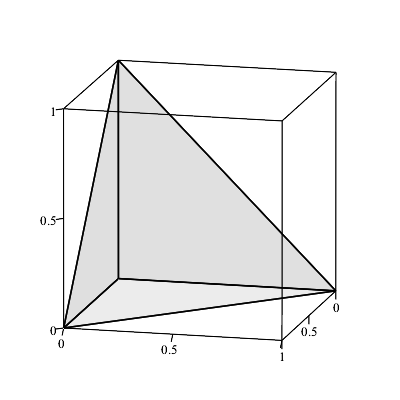
\includegraphics[trim=0.5cm 1.0cm 0.5cm 1.0cm, clip]{11_3_Tetrahedron_PA}} %crop graphics in animate trim=<left> <bottom> <right> <top>, add, clip with \includegraphics
  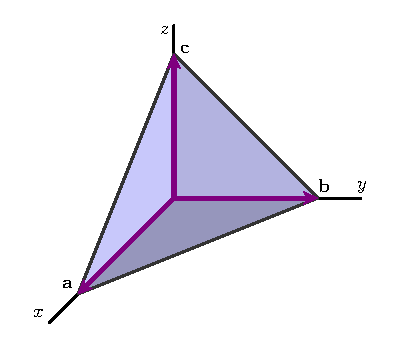
\includegraphics{figures/fig_11_3_tetrahedron.eps}
\end{center}
\caption{The tetrahedron $T$.}
\label{F:11.3.Tetrahedron_PA}
\ \vspace{0.05in} \
\end{minipage} \hspace{0.5in}
\begin{minipage}{2.5in}
\begin{center}
%\resizebox{!}{2.0in}{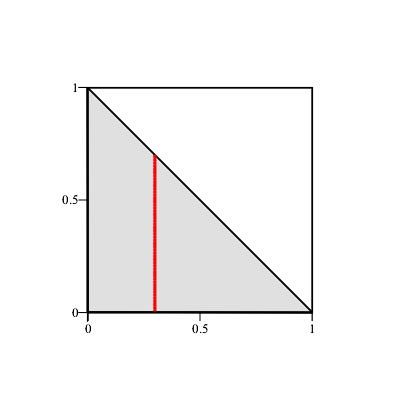
\includegraphics[trim=1.0cm 1.5cm 1.0cm 1.5cm, clip]{11_3_Tetrahedron_proj_PA}} %crop graphics in animate trim=<left> <bottom> <right> <top>, add, clip with \includegraphics
  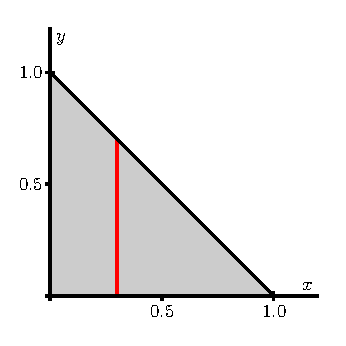
\includegraphics{figures/fig_11_3_tetra_project.eps}
\end{center}
\caption{Projecting $T$ onto the $xy$-plane.}
\label{F:11.3.Tetrahedron_proj_PA}
\end{minipage}
\end{center}
\end{figure}
    \ba
    \item Use the formula (\ref{eq:11.3.tetrahedron_volume}) to find the volume of the tetrahedron $T$.
    
    \item Instead of memorizing or looking up the formula for the volume of a tetrahedron, we can use a double integral to calculate the volume of the tetrahedron $T$. To see how, notice that the top face of the tetrahedron $T$ is the plane whose equation is
        \[z = 1-(x+y).\]
        Provided that we can use an iterated integral on a non-rectangular region, the volume of the tetrahedron will be given by an iterated integral of the form
        \[\int_{x=?}^{x=?} \int_{y=?}^{y=?} 1-(x+y) \, dy \, dx.\]
        The issue that is new here is how we find the limits on the integrals; note that the outer integral's limits are in $x$, while the inner ones are in $y$, since we have chosen $dA = dy \, dx$. To see the domain over which we need to integrate, think of standing way above the tetrahedron looking straight down on it, which means we are projecting the entire tetrahedron onto the $xy$-plane. The resulting domain is the triangular region shown in Figure \ref{F:11.3.Tetrahedron_proj_PA}. \\

Explain why we can represent the triangular region with the inequalities
        \[0 \leq y \leq 1-x \ \ \ \text{ and } \ \ \ 0 \leq x \leq 1.\]
        (Hint: Consider the cross sectional slice shown in Figure \ref{F:11.3.Tetrahedron_proj_PA}.)


\item Explain why it makes sense to now write
the volume integral in the form
        \[\int_{x=?}^{x=?} \int_{y=?}^{y=?} 1-(x+y) \, dy \, dx = \int_{x=0}^{x=1} \int_{y=0}^{y=1-x} 1-(x+y) \, dy \, dx. \]

\item Use the Fundamental Theorem of Calculus to evaluate the iterated integral
        \[\int_{x=0}^{x=1} \int_{y=0}^{y=1-x} 1-(x+y) \, dy \, dx\]
        and compare to your result from part (a).  (As with iterated integrals over rectangular regions, start with the inner integral.)

    \ea

\end{pa} 


\begin{activitySolution}

    \ba
    \item Let $O=(0,0,0)$, $P=(1,0,0)$, $Q=(0,1,0)$, and $R=(0,0,1)$. With these points as the vertices of the tetrahedron we have
 \[\va = \langle 1,0,0 \rangle, \ \ \ \vb = \langle 0,1,0 \rangle, \ \ \ \text{ and } \ \ \ \vc = \langle 0,0,1 \rangle,.\]
Using the formula we obtain
\begin{align*}
\frac{\va \cdot (\vb \times \vc)}{6} &= \frac{\vi \cdot (\vj \times \vk)}{6} \\
    &= \frac{\vi \cdot \vi}{6} \\
    &= \frac{1}{6}.
\end{align*}


    \item If we take a cross section of the domain for a fixed value of $x$ as shown in Figure \ref{F:11.3.Tetrahedron_proj_PA}, we can see that the $y$ values on the cross section all have a lowest value of 0, but their highest values lie on the line $y=1-x$. We can construct these cross sections for any value of $x$ between 0 and 1, so this triangular region is described by the inequalities $0 \leq y \leq 1-x$ and $0 \leq x \leq 1$.


\item When we slice vertically, each slice runs from the $x$-axis to the line $y=1-x$. So the limits on $y$ are $0 \leq y \leq 1-x$. The triangular region has $x$ values that run from $0$ to $1$, so the limits on the integral as as shown. 

\item Using basic integration techniques we have
\begin{align*}
\int_{0}^{1} \int_{0}^{1-x} 1-(x+y) \, dy \, dx &= \int_0^1 \left(y - xy - \frac{y^2}{2} \right)\biggm|_0^{1-x} \, dx \\
    &= \int_0^1 (1-x) - x(1-x) - \frac{1}{2}(1-x)^2 \, dx \\
    &= \frac{1}{2} \int_0^1 x^2-2x+1 \, dx \\
    &= \frac{1}{2}\left(\frac{x^3}{3} - x^2 + x \right)\biggm|_0^1 \\
    &= \frac{1}{2}\left(\frac{1}{3}\right) \\
    &= \frac{1}{6}.
\end{align*}
This is the same result we obtained from the formula in part (a).


    \ea

\end{activitySolution}

\afterpa 

\subsection*{Double Integrals over General Regions}

So far, we have learned that a double integral over a rectangular region may be interpreted in one of two ways:
\begin{itemize}
\item $\ds \iint_R f(x,y) \, dA$ tells us the volume of the solids the graph of $f$ bounds above the $xy$-plane over the rectangle $R$ minus the volume of the solids the graph of $f$ bounds below the $xy$-plane under the rectangle $R$;
\item $\ds \frac{1}{A(R)} \iint_R f(x,y) \, dA$, where $A(R)$ is the area of $R$ tells us the average value of the function $f$ on $R$. If $f(x, y) \geq  0$ on $R$, we can interpret this average value of $f$ on $R$ as the height of the box with base $R$ that has the same volume as the volume of the surface defined by $f$ over $R$.
\end{itemize}

As we saw in Preview Activity~\ref{PA:11.1}, a function $f = f(x,y)$ may be considered over regions other than rectangular ones, and thus we want to understand how to set up and evaluate double integrals over non-rectangular regions.  Note that if we can, then the two interpretations of the double integral noted above will naturally extend to solid regions with non-rectangular bases.

So, suppose $f$ is a continuous function on a closed, bounded domain $D$. For example, consider $D$ as the circular domain shown in Figure \ref{F:11.3.nonrect_domain_1}.
\begin{figure}[ht]
\begin{center}
\begin{minipage}{2.5in}
\begin{center}
%\resizebox{!}{0.75in}{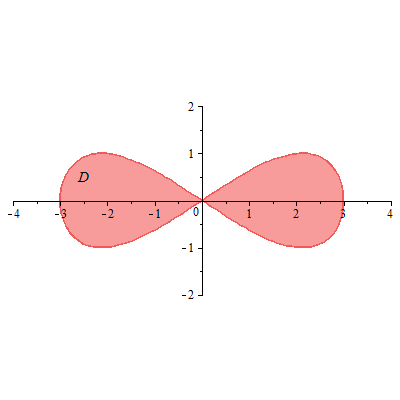
\includegraphics[trim=0cm 5cm 0cm 5cm, clip]{11_3_nonrect_1}} %crop graphics in animate trim=<left> <bottom> <right> <top>, add, clip with \includegraphics
  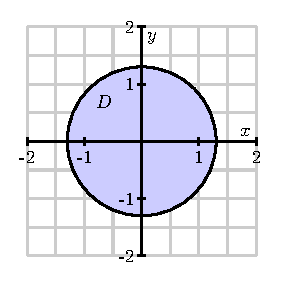
\includegraphics{figures/fig_11_3_circular.eps}
\end{center}
\caption{A non-rectangular domain.}
\label{F:11.3.nonrect_domain_1}
\end{minipage} \hspace{0.5in}
\begin{minipage}{2.5in}
\begin{center}
%\resizebox{!}{0.75in}{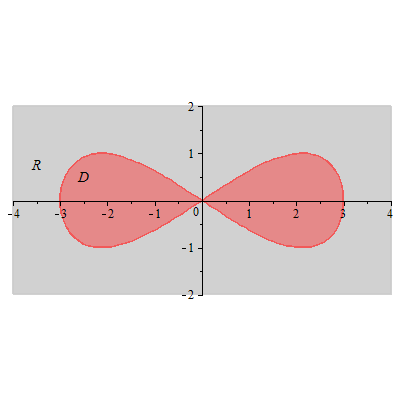
\includegraphics[trim=0cm 5cm 0cm 5cm, clip]{11_3_nonrect_2}}
  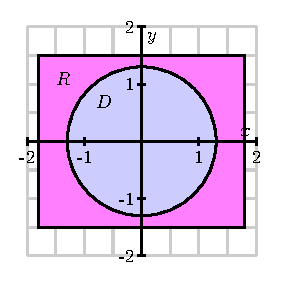
\includegraphics{figures/fig_11_3_circular_rect.eps}
\end{center}
\caption{Enclosing this domain in a rectangle.}
\label{F:11.3.nonrect_domain_2}
\end{minipage}
\end{center}
\end{figure}
We can enclose $D$ in a rectangular domain $R$ as shown in Figure \ref{F:11.3.nonrect_domain_2} and extend the function $f$ to be defined over $R$ in order to be able to use the definition of the double integral over a rectangle.  We extend $f$ in such a way that its values at the points in $R$ that are not in $D$ contribute 0 to the value of the integral. In other words, define a function $F = F(x, y)$ on $R$ as
\[F(x,y) = \begin{cases} f(x,y), &\text{ if } (x,y) \in D, \\ 0, &\text{ if } (x,y) \not\in D \end{cases}.\]
We then say that the double integral of $f$ over $D$\index{double integral over a general region} is the same as the double integral of $F$ over $R$, and thus
\[\iint_D f(x,y) \, dA = \iint_R F(x,y) \, dA.\]
In practice, we just ignore everything that is in $R$ but not in $D$, since these regions contribute 0 to the value of the integral.

Just as with double integrals over rectangles, a double integral over a domain $D$ can be evaluated as an iterated integral.  If the region $D$ can be described by the inequalities $g_1(x) \leq y \leq g_2(x)$ and $a \leq x \leq b$, where $g_1=g_1(x)$ and $g_2=g_2(x)$ are functions of only $x$, then  
\[\iint_D f(x,y) \, dA = \int_{x=a}^{x=b} \int_{y=g_1(x)}^{y=g_2(x)} f(x,y) \, dy \, dx.\]
Alternatively, if the region $D$ is described by the inequalities $h_1(y) \leq x \leq h_2(y)$ and $c \leq y \leq d$, where $h_1=h_1(y)$ and $h_2=h_2(y)$ are functions of only $y$, we have
\[\iint_D f(x,y) \, dA = \int_{y=c}^{y=d} \int_{x=h_1(y)}^{x=h_2(y)} f(x,y) \, dx \, dy.\]

The structure of an iterated integral is of particular note:

\vspace*{5pt}
\nin \framebox{\hspace*{3 pt}
\parbox{6.25 in}{In an iterated double integral:
\begin{itemize}
\item the limits on the outer integral must be constants;
\item the limits on the inner integral must be constants or in terms of only the remaining variable -- that is, if the inner integral is with respect to $y$, then its limits may only involve $x$ and constants, and vice versa.
\end{itemize}
} \hspace*{3 pt}}
\vspace*{5pt}

We next consider a detailed example.

\begin{example} Let $f(x,y) = x^2y$ be defined on the triangle $D$ with vertices $(0,0)$, $(2,0)$, and $(2,3)$ as shown in Figure \ref{F:11.3.DI_1}.
\begin{figure}[h]
\begin{center}
\begin{minipage}{1.75in}
\begin{center}
%\resizebox{!}{1.25in}{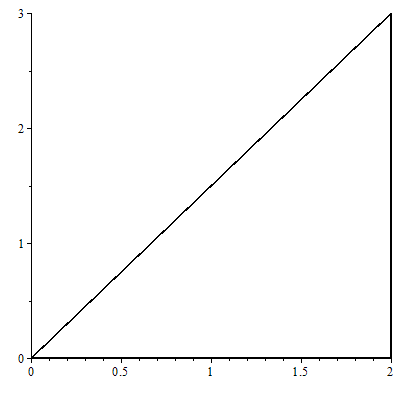
\includegraphics{11_3_DI_1}}
  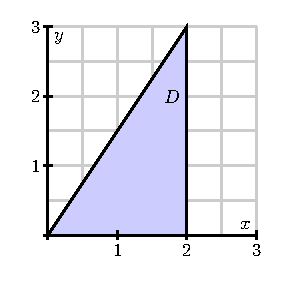
\includegraphics{figures/fig_11_3_triangular.eps}
\end{center}
\caption{A triangular domain.}
\label{F:11.3.DI_1}
\end{minipage} \hspace{0.2in}
\begin{minipage}{1.75in}
\begin{center}
%\resizebox{!}{1.25in}{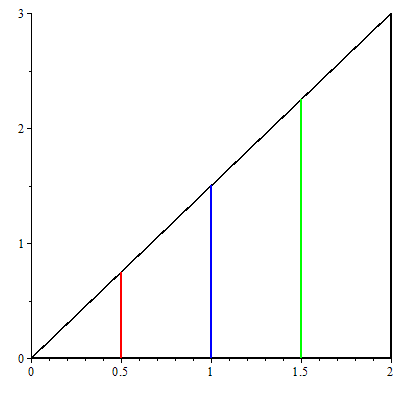
\includegraphics{11_3_DI_1y}}
  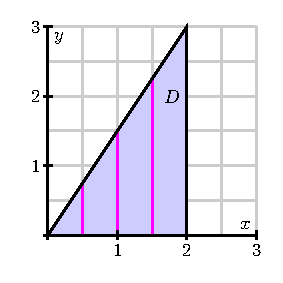
\includegraphics{figures/fig_11_3_triangular_v.eps}
\end{center}
\caption{Slices in the $y$ direction.}
\label{F:11.3.DI_1y}
\end{minipage}
\hspace{0.2in}
\begin{minipage}{1.75in}
\begin{center}
%\resizebox{!}{1.25in}{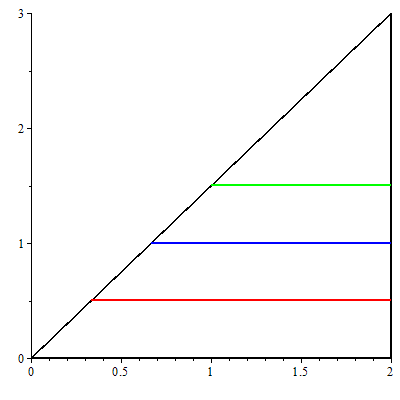
\includegraphics{11_3_DI_1x}}
  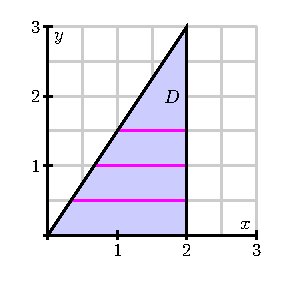
\includegraphics{figures/fig_11_3_triangular_h.eps}
\end{center}
\caption{Slices in the $x$ direction.}
\label{F:11.3.DI_1x}
\end{minipage}
\end{center}
\end{figure}
To evaluate $\ds \iint_D f(x,y) \, dA$, we must first describe the region $D$ in terms of the variables $x$ and $y$. We take two approaches.
\begin{description}
\item[Approach 1: Integrate first with respect to $y$.] In this case we choose to evaluate the double integral as an iterated integral in the form
\[\iint_D x^2y \, dA = \int_{x=a}^{x=b} \int_{y=g_1(x)}^{y=g_2(x)} x^2y \, dy \, dx,\]
and therefore we need to describe $D$ in terms of inequalities
\[g_1(x) \leq y \leq g_2(x) \ \ \ \ \ \text{ and} \ \ \ \ \ a \leq x \leq b.\]
Since we are integrating with respect to $y$ first, the iterated integral has the form
\[ \iint_D x^2y \, dA =\int_{x=a}^{x=b} A(x) \, dx,\]
where $A(x)$ is a cross sectional area in the $y$ direction. So we are slicing the domain perpendicular to the $x$-axis and want to understand what a cross sectional area of the overall solid will look like. Several slices of the domain are shown in Figure \ref{F:11.3.DI_1y}. On a slice with fixed $x$ value, the $y$ values are bounded below by 0 and above by the $y$ coordinate on the hypotenuse of the right triangle. Thus, $g_1(x) = 0$;  to find $y = g_2(x)$, we need to write the hypotenuse as a function of $x$. The hypotenuse connects the points (0,0) and (2,3) and hence has equation $y = \frac{3}{2}x$. This gives the upper bound on $y$ as $g_2(x) = \frac{3}{2}x$. The leftmost vertical cross section is at $x=0$ and the rightmost one is at $x=2$, so we have $a=0$ and $b=2$. Therefore,
\[\iint_D x^2y \, dA = \int_{x=0}^{x=2} \int_{y=0}^{y = \frac32 x} x^2y \, dy \, dx.\]
We evaluate the iterated integral by applying the Fundamental Theorem of Calculus first to the inner integral, and then to the outer one, and find that
\begin{align*}
\int_{x=0}^{x=2} \int_{y=0}^{y=\frac32 x} x^2y \, dy \, dx &= \int_{x=0}^{x=2} \left[x^2 \cdot \frac{y^2}{2}\right]\biggm|_{y=0}^{y=\frac32 x} \, dx \\
	&= \int_{x=0}^{x=2} \frac{9}{8}x^4\, dx \\
	&= \frac{9}{8}\frac{x^5}{5}\biggm|_{x=0}^{x=2} \\
	&= \left(\frac{9}{8}\right) \left(\frac{32}{5}\right) \\
	&= \frac{36}{5}.
\end{align*}

%\begin{figure}[h]
%\begin{center}
%\resizebox{!}{1.5in}{\includegraphics{DI_1}} \hspace{1.0in} \resizebox{!}{1.5in}{\includegraphics{DI_1x}}
%\end{center}
%\caption{{\scriptsize Left: A triangular domain. Right: Cross sectional slices in the $x$ direction.}}
%\label{F:11.3.DI_2}
%\end{figure}

\item[Approach 2: Integrate first with respect to $x$.] In this case, we choose to evaluate the double integral as an iterated integral in the form
\[\iint_D x^2y \, dA = \int_{y=c}^{y=d} \int_{x=h_1(y)}^{x=h_2(y)} x^2y \, dx \, dy\]
and thus need to describe $D$ in terms of inequalities
\[h_1(y) \leq x \leq h_2(y) \ \ \ \ \ \text{ and }  \ \ \ \ \  c \leq y \leq d.\]
Since we are integrating with respect to $x$ first, the iterated integral has the form
\[ \iint_D x^2y \, dA = \int_c^d A(y) \, dy,\]
where $A(y)$ is a cross sectional area of the solid in the $x$ direction.  Several slices of the domain -- perpendicular to the $y$-axis -- are shown in Figure \ref{F:11.3.DI_1x}.

On a slice with fixed $y$ value, the $x$ values are bounded below by the $x$ coordinate on the hypotenuse of the right triangle and above by 2. So $h_2(y) = 2$; to find $h_1(y)$, we need to write the hypotenuse as a function of $y$. Solving the earlier equation we have for the hypotenuse ($y = \frac32 x$) for $x$ gives us $x = \frac{2}{3}y$. This makes $h_1(y) = \frac{2}{3}y$. The lowest horizontal cross section is at $y=0$ and the uppermost one is at $y=3$, so we have $c=0$ and $d=3$. Therefore,
\[\iint_D x^2y \, dA = \int_{y=0}^{y=3} \int_{x=(2/3)y}^{x=2} x^2y \, dx \, dy.\]
We evaluate the resulting iterated integral as before by twice applying the Fundamental Theorem of Calculus, and find that
\begin{align*}
\int_{y=0}^{y=3} \int_{x=\frac{2}{3}y}^{2} x^2y \, dx \, dy &= \int_{y=0}^{y=3} \left[\frac{x^3}{3}\right]\biggm|_{x=\frac{2}{3}y}^{x=2}y \, dx \\
	&= \int_{y=0}^{y=3} \left[\frac{8}{3}y - \frac{8}{81}y^4 \right] \, dy \\
	&= \left[\frac{8}{3}\frac{y^2}{2} - \frac{8}{81}\frac{y^5}{5}\right]\biggm|_{y=0}^{y=3} \\
	&= \left(\frac{8}{3}\right) \left(\frac{9}{2}\right) - \left(\frac{8}{81}\right) \left(\frac{243}{5}\right) \\
	&= 12 - \frac{24}{5} \\
	&= \frac{36}{5}.
\end{align*}
\end{description}
We see, of course, that in the situation where $D$ can be described in two different ways, the order in which we choose to set up and evaluate the double integral doesn't matter, and the same value results in either case.

\end{example}

The meaning of a double integral over a non-rectangular region, $D$, parallels the meaning over a rectangular region.  In particular,
\begin{itemize}
\item $\ds \iint_D f(x,y) \, dA$ tells us the volume of the solids the graph of $f$ bounds above the $xy$-plane over the closed, bounded region $D$ minus the volume of the solids the graph of $f$ bounds below the $xy$-plane under the region $D$;
\item $\ds \frac{1}{A(D)} \iint_R f(x,y) \, dA$, where $A(D)$ is the area of $D$ tells us the average value of the function $f$ on $D$. If $f(x, y) \geq  0$ on $D$, we can interpret this average value of $f$ on $D$ as the height of the solid with base $D$ and constant cross-sectional area $D$ that has the same volume as the volume of the surface defined by $f$ over $D$.
\end{itemize}

\begin{activity} \label{A:11.3.1}  Consider the double integral $\ds \iint_D (4-x-2y) \, dA$, where $D$ is the triangular region with vertices (0,0), (4,0), and (0,2).
		\ba
		\item Write the given integral as an iterated integral of the form $\ds \iint_D (4-x-2y) \, dy \, dx$. Draw a labeled picture of $D$ with relevant cross sections.

		\item Write the given integral as an iterated integral of the form $\ds \iint_D (4-x-2y) \, dx \, dy$. Draw a labeled picture of $D$ with relevant cross sections.

		\item Evaluate the two iterated integrals from (a) and (b), and verify that they produce the same value. Give at least one interpretation of the meaning of your result.

	\ea

\end{activity}
\begin{smallhint}

\end{smallhint}
\begin{bighint}

\end{bighint}
\begin{activitySolution}
\ba
		\item Integrating with respect to $y$ first means we take cross sections of $D$ parallel to the $y$-axis. As the figure below illustrates, the lower end of any cross section is always on the $x$-axis (with $y=0$) and the upper limit is on the line joining $(4,0)$ and $(0,2)$. The limits on $y$ need to written in terms of $x$, so the upper limit is $y = 2-\frac{1}{2}x$. These cross sections run from $x=0$ to $x=4$, so as an iterated integral we have 
\[\iint_D \left(\frac{3}{4}\right)(4-x-2y) \, dy \, dx = \int_{0}^{4} \int_{0}^{2-(1/2)x} \left(\frac{3}{4}\right)(4-x-2y) \, dy \, dx.\]

%Shift up 0.5 to leave space for the x-labels
\begin{center}
\setlength{\unitlength}{1.0cm}
\begin{picture}(4.5,3.0)
\linethickness{0.35mm}
\put(0,0.5){\vector(1,0){4.5}}
\put(0,0.5){\vector(0,1){2.5}}
\color{red}
\put(0,2.5){\line(2,-1){4.0}}
\color{black}
\put(4.4,0.2){$x$}
\put(-0.3,2.9){$y$}
\put(1,0.4){\line(0,1){0.2}}
\put(2,0.4){\line(0,1){0.2}}
\put(3,0.4){\line(0,1){0.2}}
\put(4,0.4){\line(0,1){0.2}}
\put(-0.1,1.5){\line(1,0){0.2}}
\put(-0.1,2.5){\line(1,0){0.2}}
\put(3.9,0){$4$}
\put(-0.4,2.4){$2$}
\put(2,1.7){$y=2-\frac{1}{2}x$}

\color{blue}
\linethickness{0.35mm}
\put(0.2,0.5){\line(0,1){1.9}}
\put(1.2,0.5){\line(0,1){1.4}}
\put(2.2,0.5){\line(0,1){0.9}}
\put(3.2,0.5){\line(0,1){0.4}}
\end{picture}
\end{center}


		\item Integrating with respect to $x$ first means we take cross sections of $D$ parallel to the $x$-axis. As the figure below illustrates, the lower end of any cross section is always on the $y$-axis (with $x=0$) and the upper limit is on the line joining $(4,0)$ and $(0,2)$. The limits on $x$ need to written in terms of $y$, so the upper limit is $x = 4-2y$. These cross sections run from $y=0$ to $y=2$, so as an iterated integral we have 
\[\iint_D \left(\frac{3}{4}\right)(4-x-2y) \, dx \, dy = \int_{0}^{2} \int_{0}^{4-2y} \left(\frac{3}{4}\right)(4-x-2y) \, dx \, dy.\]

\begin{center}
\setlength{\unitlength}{1.0cm}
\begin{picture}(4.5,3.0)
\linethickness{0.35mm}
\put(0,0.5){\vector(1,0){4.5}}
\put(0,0.5){\vector(0,1){2.5}}
\color{red}
\put(0,2.5){\line(2,-1){4.0}}
\color{black}
\put(4.4,0.2){$x$}
\put(-0.3,2.9){$y$}
\put(1,0.4){\line(0,1){0.2}}
\put(2,0.4){\line(0,1){0.2}}
\put(3,0.4){\line(0,1){0.2}}
\put(4,0.4){\line(0,1){0.2}}
\put(-0.1,1.5){\line(1,0){0.2}}
\put(-0.1,2.5){\line(1,0){0.2}}
\put(3.9,0){$4$}
\put(-0.4,2.4){$2$}
\put(2,1.7){$x=4-2y$}

\color{blue}
\linethickness{0.35mm}
\put(0,0.9){\line(1,0){3.2}}
\put(0,1.3){\line(1,0){2.4}}
\put(0,2.1){\line(1,0){0.8}}
\end{picture}
\end{center}


\item Evaluating the iterated integral with respect to $y$ then $x$ gives us  
\begin{align*}
\iint_D \left(\frac{3}{4}\right)(4-x-2y) \, dy \, dx &= \int_{0}^{4} \int_{0}^{2-(1/2)x} \left(\frac{3}{4}\right)(4-x-2y) \, dy \, dx \\
	&= \frac{3}{4} \int_{0}^{4} \left. \left[(4-x)y-y^2\right] \right|_{0}^{2-(1/2)x} \, dx \\
	&= \frac{3}{4} \int_{0}^{4}  \left[(4-x)\left(2-\frac{1}{2}x\right)-\left(2-\frac{1}{2}x\right)^2\right] \, dx \\
	&= \frac{3}{4} \int_{0}^{4}  \left[4-2x+\frac{1}{4}x^2\right] \, dx \\
	&= \frac{3}{4} \left. \left[4x-x^2+\frac{1}{12}x^3\right] \right|{0}^{4} \\
	&= \frac{3}{4} \left(\frac{16}{3}\right) \\
	&= 4.
\end{align*}
Evaluating the iterated integral with respect to $y$ then $x$ gives us 
\begin{align*}
\iint_D \left(\frac{3}{4}\right)(4-x-2y) \, dx \, dy &= \int_{0}^{2} \int_{0}^{4-2y} \left(\frac{3}{4}\right)(4-x-2y) \, dx \, dy \\
	&= \frac{3}{4} \int_{0}^{2}  \left. \left[4x-\frac{x^2}{2}-2yx \right] \right|_{0}^{4-2y} \, dy \\
	&= \frac{3}{4} \int_{0}^{2}   \left[4(4-2y)-\frac{(4-2y)^2}{2}-2y(4-2y) \right] \, dy \\
	&= \frac{3}{4} \int_{0}^{2}   \left[8-8y+2y^2 \right] \, dy \\
	&= \frac{3}{4} \left. \left[8y-4y^2+\frac{2}{3}y^3 \right] \right|_{0}^{2}  \\
	&= \frac{3}{4} \left(\frac{16}{3}\right)  \\
	&= 4.
\end{align*}
Since $f$ is non-negative on the domain $D$, these two iterated integrals tell us the volume of the solid bounded above by the graph of $f(x,y) = \frac{3}{4}(4-x-2y)$ and below by the triangular region $D$. 

\ea
\end{activitySolution}
\aftera


\begin{activity} \label{A:11.3.2} Consider the iterated integral $\ds \int_{x=3}^{x=5} \int_{y=-x}^{y=x^2} (4x+10y) \, dy \, dx$.
    \ba
    \item Sketch the region of integration, $D$, for which 
    $$\ds \iint_D (4x + 10y) \, dA = \int_{x=3}^{x=5} \int_{y=-x}^{y=x^2} (4x+10y) \, dy \, dx.$$

    \item Determine the equivalent iterated integral that results from integrating in the opposite order ($dx \, dy$, instead of $dy \, dx$).  That is, determine the limits of integration for which 
$$\ds \iint_D (4x + 10y) \, dA = \int_{y=?}^{y=?}  \int_{x=?}^{x=?} (4x+10y) \, dx \, dy.$$
    \item Evaluate one of the two iterated integrals above. Explain what the value you obtained tells you.
    
    \item Set up and evaluate a single definite integral to determine the exact area of $D$, $A(D)$.
    
    \item Determine the exact average value of $f(x,y) = 4x  + 10y$ over $D$.

    \ea

\end{activity}
\begin{smallhint}

\end{smallhint}
\begin{bighint}

\end{bighint}
\begin{activitySolution}
   \ba
    \item The region $D$ of integration has $-x \leq y \leq x^2$ and $3 \leq x \leq 5$. This region is as shown in the figure below.
\begin{center}
\resizebox{!}{2.0in}{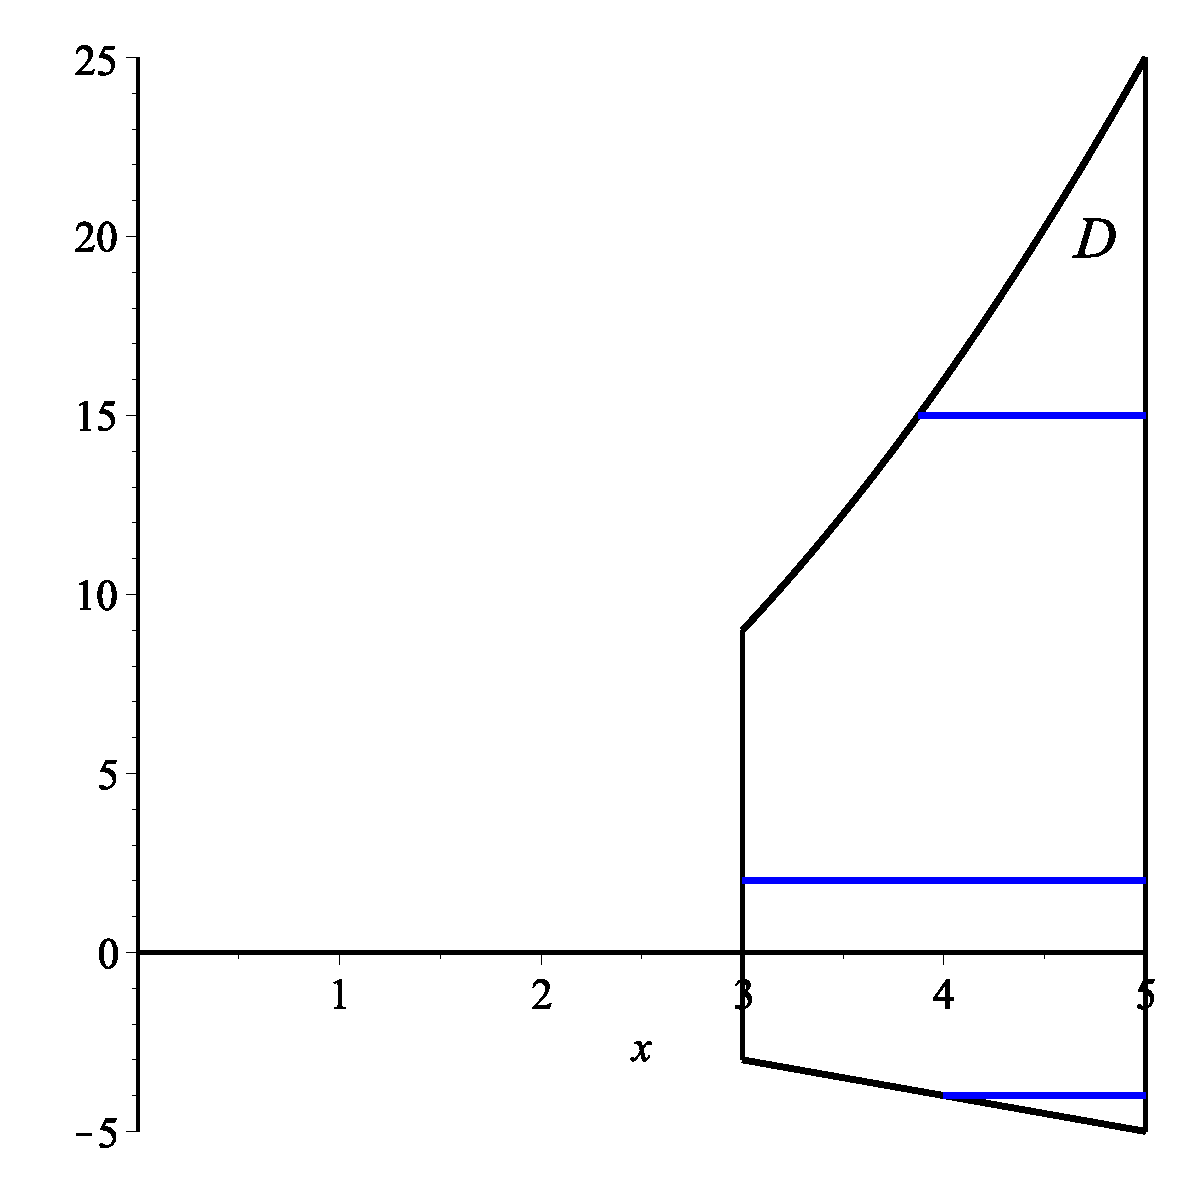
\includegraphics{11_3_Act_2}}
\end{center}


    \item If we integrate with respect to $x$ first, then $y$, the cross sections in the $x$-direction will always have their right endpoints on the line $x=5$. However, the left endpoints change as shown in the figure above. At the bottom of the figure, $x$ runs from $-y$ to $5$ for $y$ between $-3$ and $-5$. In the middle, $x$ runs between $x=3$ and $x=5$ for $y$ between $-3$ and $9$. At the top, $x$ runs from $\sqrt{y}$ to $x=5$ for $y$ between $9$ and $25$. So a sum of  iterated integrals that gives the same value as the given iterated integral is 
\[\int_{-5}^{-3} \int_{-y}^{5} (4x+10y) \, dx \, dy + \int_{-3}^{9} \int_{3}^{5} (4x+10y) \, dx \, dy + \int_{9}^{25} \int_{\sqrt{y}}^{5} (4x+10y) \, dx \, dy.\]

    \item Evaluating the original integral yields
\begin{align*}
\int_3^5 \int_{-x}^{x^2} (4x+10y) \, dy \, dx &= \int_3^5 \left. \left[4xy+5y^2\right] \right|_{-x}^{x^2} \, dx \\
	&= \int_3^5  \left[\left(4x^3+5x^4\right) - \left(-4x^2+5x^2\right)\right] \, dx \\
	&= \int_3^5  \left[5x^4+4x^3-x^2\right] \, dx \\
	&= \left. \left[x^5+x^4-\frac{x^3}{3}\right] \right|_3^5  \\
	&= \frac{11125}{3} - 315 \\
	&= \frac{10180}{3}.
\end{align*}

Since $4x+10y \geq 0$ on this domain, the value obtained tells us the volume of the solid bounded above by the graph of the plane $4x+10y$ and below by the region of integration. 

\item The area of $D$ is found by integrating 1 over the domain $D$, or
\begin{align*}
A(D) &= \iint_D 1 \, dA \\
	&= \int_{x=3}^{x=5} \int_{y=-x}^{y=x^2} 1 \, dy \, dx \\
	&= \int_3^5  \left[x^2+x\right] \, dx \\
	&= \left. \left[\frac{x^3}{3}+\frac{x^2}{2}\right] \right|_3^5  \\
	&= \left[\frac{125}{3} + \frac{25}{2}\right] - \left[\frac{27}{3}+\frac{9}{2}\right] \\
	&= \frac{122}{3}.
\end{align*}

\item The average value of $f$ on $D$ is 
\[\frac{1}{A(D)} \iint_D f(x,y) \, dA = \frac{3}{122}\left(\frac{10180}{3}\right) = \frac{5090}{61}.\]

    \ea
\end{activitySolution}
\aftera


\begin{activity} \label{A:11.3.3} Consider the iterated integral $\ds \int_{x=0}^{x=4} \int_{y=x/2}^{y=2} e^{y^2} \, dy \, dx$.

\ba
  \item Explain why we cannot antidifferentiate $e^{y^2}$ with respect to $y$, and thus are unable to evaluate the iterated integral $\ds  \int_{x=0}^{x=4} \int_{y=x/2}^{y=2} e^{y^2} \, dy \, dx$ using the Fundamental Theorem of Calculus. 
  \item Sketch the region of integration, $D$, so that $\ds \iint_D e^{y^2} \, dA = \int_{x=0}^{x=4} \int_{y=x/2}^{y=2} e^{y^2} \, dy \, dx.$
  \item Rewrite the given iterated integral in the opposite order, using $dA = dx \, dy$.
  \item Use the Fundamental Theorem of Calculus to evaluate the iterated integral you developed in (d).  Write one sentence to explain the meaning of the value you found.
  \item What is the important lesson this activity offers regarding the order in which we set up an iterated integral?
\ea

\end{activity}
\begin{smallhint}

\end{smallhint}
\begin{bighint}

\end{bighint}
\begin{activitySolution}
\ba
\item No substitution will work to integrate $e^{y^2}$ because of the square in the exponent. Using parts only makes the integral more complicated, and we have no other techniques to apply to this integrand.

\item The domain $D$ of integration is shown below. 
%Shift up 0.5 to leave space for the x-labels
\begin{center}
\setlength{\unitlength}{1.0cm}
\begin{picture}(4.5,3.0)
\linethickness{0.35mm}
\put(0,0.5){\vector(1,0){4.5}}
\put(0,0.5){\vector(0,1){2.5}}
\put(0,2.5){\line(1,0){4}}
\color{red}
\put(0,0.5){\line(2,1){4.0}}
\color{black}
\put(4.4,0.2){$x$}
\put(-0.3,2.9){$y$}
\put(1,0.4){\line(0,1){0.2}}
\put(2,0.4){\line(0,1){0.2}}
\put(3,0.4){\line(0,1){0.2}}
\put(4,0.4){\line(0,1){0.2}}
\put(-0.1,1.5){\line(1,0){0.2}}
\put(-0.1,2.5){\line(1,0){0.2}}
\put(3.9,0){$4$}
\put(-0.4,2.4){$2$}
\put(2.5,1.5){$y=\frac{x}{2}$}

\color{blue}
\linethickness{0.35mm}
\put(0,1.0){\line(1,0){1.0}}
\put(0,2.0){\line(1,0){3.0}}
\end{picture}
\end{center}

\item When we first integrate with respect to $x$, we can see that the cross sections go from $x=0$ to $x = 2y$. The limits on $y$ are then $0$ to $2$, giving us
\[\iint_D e^{y^2} \, d = \int_0^2 \int_{0}^{2y} e^{y^2} \, dx \, dy.\]

\item Evaluating the iterated integral yields 
\begin{align*}
\int_0^4 \int_{0}^{x/2} e^{y^2} \, dy \, dx &= \int_0^2 \int_{0}^{2y} e^{y^2} \, dx \, dy \\
	&= \int_0^2 \left. xe^{y^2} \right|_{0}^{2y} \, dy \\
	&= \int_0^2 2ye^{y^2} \, dy \\
	&= \left. e^{y^2} \right|_0^2 \\
	&= e^4-1.
\end{align*}
Since $e^{y^2} > 0$ on $D$, this integral tells us the volume of the solid bounded above by the surface $z=e^{y^2}$ and below by the region $D$. 

\item We need to be flexible when setting up iterated integrals -- sometimes one order of integration is very difficult (or impossible) while the other order is easier. So it is important to practice changing the order of integration in iterated integrals. 

\ea

\end{activitySolution}

\aftera



\begin{summary}
\item For a double integral $\ds \iint_D f(x,y) \, dA$ over a non-rectangular region $D$, we enclose $D$ in a rectangle $R$ and then extend integrand $f$ to a function $F$ so that $F(x,y) = 0$ at all points in $R$ outside of $D$ and $F(x,y) = f(x,y)$ for all points in $D$. We then define $\ds \iint_D f(x,y) \, dA$ to be equal to $\ds \iint_R F(x,y) \, dA$.
\item In an iterated double integral, the limits on the outer integral must be constants while the limits on the inner integral must be constants or in terms of only the remaining variable. In other words, an iterated double integral has one of the following forms (which result in the same value):
\[\int_{x=a}^{x=b} \int_{y=g_1(x)}^{y=g_2(x)} f(x,y) \, dy \, dx,\]
where $g_1=g_1(x)$ and $g_2=g_2(x)$ are functions of $x$ only and the region $D$ is described by the inequalities $g_1(x) \leq y \leq g_2(x)$ and $a \leq x \leq b$ or
\[\int_{y=c}^{y=d} \int_{x=h_1(y)}^{x=h_2(y)} f(x,y) \, dx \, dy,\]
where $h_1=h_1(y)$ and $h_2=h_2(y)$ are functions of $y$ only and the region $D$ is described by the inequalities $h_1(y) \leq x \leq h_2(y)$ and $c \leq y \leq d$.
\end{summary}



\nin \hrulefill

\begin{exercises} 

\item For each of the following iterated integrals, (a) sketch the region of integration, (b) write an equivalent iterated integral expression in the opposite order of integration, and (c) choose one of the two orders and evaluate the integral.
\ba
	\item $\ds \int_{x=0}^{x=1}  \int_{y=x^2}^{y=x} xy \, dy  \, dx$
	\item $\ds \int_{y=0}^{y=2}  \int_{x=-\sqrt{4-y^2}}^{x=0} xy \, dx  \, dy$
	\item $\ds \int_{x=0}^{x=1}  \int_{y=x^4}^{y=x^{1/4}} x+y \, dy  \, dx$
	\item $\ds \int_{y=0}^{y=2}  \int_{x=y/2}^{x=2y} x+y \, dx  \, dy$
\ea

\begin{exerciseSolution}
\ba
	\item Integrating in the reverse order gives us 
\[\int_{y=0}^{y=1}  \int_{x=y}^{x=\sqrt{y}} xy \, dy  \, dx.\]

We integrate first with respect to $y$:
\begin{align*}
\int_{x=0}^{x=1}  \int_{y=x^2}^{y=x} xy \, dy  \, dx &= \int_{x=0}^{x=1} \frac{1}{2}xy^2 \biggm|_{y=x^2}^{y=x}  \, dx \\
	&= \int_{x=0}^{x=1} \frac{1}{2}x\left(x^2-x^4\right) \, dx \\
	&= \int_{x=0}^{x=1} \frac{1}{2}\left(x^3-x^5\right) \, dx \\
	&= \frac{1}{2} \left(\frac{1}{4}x^4-\frac{1}{6}x^6\right)\biggm|_{x=0}^{x=1} \\
	&= \frac{1}{2} \left(\frac{1}{4}-\frac{1}{6}\right) \\
	&= \frac{1}{24}.
\end{align*}

	\item Integrating in the reverse order gives us 
\[\int_{x=-2}^{x=0}  \int_{y=0}^{y=\sqrt{4-x^2}} xy \, dy  \, dx.\]

We integrate first with respect to $y$:
\begin{align*}
\int_{x=-2}^{x=0}  \int_{y=0}^{y=\sqrt{4-x^2}} xy \, dy  \, dx &= \int_{x=-2}^{x=0} \frac{1}{2}xy^2 \biggm|_{y=0}^{y=\sqrt{4-x^2}}  \, dx \\
	&= \frac{1}{2} \int_{x=-2}^{x=0} x\left(4-x^2\right) \, dx \\
	&= \frac{1}{2}\int_{x=-2}^{x=0} \left(4x-x^3\right) \, dx \\
	&= \frac{1}{2} \left(2x^2-\frac{1}{4}x^4\right)\biggm|_{x=-2}^{x=0} \\
	&= -\frac{1}{2} \left(8-4\right) \\
	&= -2.
\end{align*}

	\item Integrating in the reverse order gives us 
\[\int_{y=0}^{y=1}  \int_{x=y^{4}}^{x=y^{1/4}} x+y \, dx  \, dy.\]

We integrate first with respect to $y$:
\begin{align*}
\int_{x=0}^{x=1}  \int_{y=x^4}^{y=x^{1/4}} x+y \, dy  \, dx &= \int_{x=0}^{x=1} \left(xy + \frac{1}{2}y^2 \right) \biggm|_{y=x^4}^{y=x^{1/4}}  \, dx \\
	&= \int_{x=0}^{x=1} x\left(x^{1/4}-x^4\right) - \frac{1}{2}\left(x^{1/2}-x^8\right) \, dx \\
	&= \int_{x=0}^{x=1} \left(x^{5/4}-x^5\right) - \frac{1}{2}\left(x^{1/2}-x^8\right) \, dx \\
	&=\left(\frac{4}{9}x^{9/4} - \frac{1}{6}x^6 - \frac{1}{3}x^{3/2} - \frac{1}{18}x^9\right)\biggm|_{x=0}^{x=1} \\
	&= \frac{4}{9} - \frac{1}{6} - \frac{1}{3} - \frac{1}{18} \\
	&= \frac{5}{9}.
\end{align*}

	\item To integrate in the reverse order we need two integrals:
\[\int_{y=x/2}^{y=2x}  \int_{x=0}^{x=1} x+y \, dy  \, dx + \int_{y=x/2}^{y=2}  \int_{x=1}^{x=4} x+y \, dy  \, dx.\]

We integrate first with respect to $x$:
\begin{align*}
\int_{y=0}^{y=2}  \int_{x=y/2}^{x=2y} x+y \, dx  \, dy &= \int_{y=0}^{y=2} \left(\frac{1}{2}x^2 +xy\right) \biggm|_{x=y/2}^{x=2y}  \, dx \\
	&= \int_{y=0}^{y=2} \left[\left(2y^2+2y^2\right) - \left(\frac{1}{8}y^2 + \frac{1}{2}y^2\right)\right] \, dy \\
	&= \frac{27}{8} \int_{y=0}^{y=2} y^2 \, dy \\
	&= \frac{27}{8} \left(\frac{1}{3}y^3\right)\biggm|_{y=0}^{y=2} \\
	&= \frac{9}{8}(8) \\
	&= 9.
\end{align*}

\ea
\end{exerciseSolution}

\item The temperature at any point on a metal plate in the $xy$ plane is given by $T(x,y) = 100-4x^2 - y^2$, where $x$ and $y$ are measured in inches and $T$ in degrees Celsius.  Consider the portion of the plate that lies on the region $D$ that is the finite region that lies between the parabolas $x = y^2$ and $x = 3 - 2y^2$.

\ba
	\item Construct a labeled sketch of the region $D$.
	\item Set up an integrated integral whose value is $\iint_D T(x,y) \, dA$. 
	\item Set up an integrated integral whose value is $\iint_D T(x,y) \, dA$.
	\item Use the Fundamental Theorem of Calculus to evaluate the integrals you determined in (b) and (c).
	\item Determine the exact average temperature, $T_{\mbox{\tiny{AVG}(D)}}$, over the region $D$.
\ea

\begin{exerciseSolution}
\ba
	\item Use appropriate technology to draw the surface. 
	\item The area of $D$ is given by 
\[A(D) = \int_{y=-1}^{y=1}  (3-2y^2) - y^2 \, dy.\]

	\item An integrated integral whose value is $\iint_D T(x,y) \, dA$ is
\[\int_{y=-1}^{y=1} \int_{x=y^2}^{x=3-2y^2} 100-4x^2 - y^2 \, dx \, dy.\]
 
	\item The area of $D$ is 
\begin{align*}
\int_{y=-1}^{y=1}  (3-2y^2) - y^2 \, dy &= \left(3y-y^3 \right)\biggm|_{y=-1}^{y=1} \\
	&= (3-1)-((-3)-(-1)) \\
	&= 4.
\end{align*}
The value of $\iint_D T(x,y) \, dA$ is
\begin{align*}
\int_{y=-1}^{y=1} \int_{x=y^2}^{x=3-2y^2} 100-4x^2 - y^2 \, dx \, dy &= \int_{y=-1}^{y=1} \left[(100-y^2)x - \frac{4}{3}x^3\right] \biggm|_{x=y^2}^{x=3-2y^2}  \, dy \\
	&= \int_{y=-1}^{y=1} \left[(100-y^2)(3-3y^2) - \frac{4}{3}\left(3-2y^2\right)^3 + \frac{4}{3}y^6\right]  \, dy \\
	&= \int_{y=-1}^{y=1} \left[264-231y^2-45y^4+12y^6\right]  \, dy \\
	&= \left[264y-77y^3-9y^5+\frac{12}{7}y^7\right] \biggm|_{y=-1}^{y=1}  \\
	&= \left[264-77-9+\frac{12}{7}\right] - \left[-264y+77+9-\frac{12}{7}\right]   \\
	&= \frac{2516}{7}.
\end{align*}

	\item The exact average temperature, $T_{\mbox{\tiny{AVG}(D)}}$, over the region $D$ is
\[T_{\mbox{\tiny{AVG}(D)}} = \frac{1}{\text{Area}(D)} \iint_D T(x,y) \, dA = \frac{2516}{28}.\]

\ea
\end{exerciseSolution}

\item Consider the solid that is given by the following description:  the base is the given region $D$, while the top is given by the surface $z = p(x,y)$.  In each setting below, set up, but do not evaluate, an iterated integral whose value is the exact volume of the solid.  Include a labeled sketch of $D$ in each case.

\ba
	\item $D$ is the interior of the quarter circle of radius 2, centered at the origin, that lies in the second quadrant of the plane; $p(x,y) = 16-x^2-y^2$.
	\item $D$ is the finite region between the line $y = x + 1$ and the parabola $y = x^2$; \\ $p(x,y) = 10-x-2y$.
	\item $D$ is the triangular region with vertices $(1,1)$, $(2,2)$, and $(2,3)$; $p(x,y) = e^{-xy}$.
	\item $D$ is the region bounded by the $y$-axis, $y = 4$ and $x = \sqrt{y}$; $p(x,y) = \sqrt{1 + x^2 + y^2}$.
\ea

\begin{exerciseSolution}
\ba
	\item The volume of the solid bounded above by the graph of $p$ and below by the region $D$ is given by 
\[\int_{x=-2}^{x=0} \int_{y=0}^{y=\sqrt{4-x^2}} 16-x^2-y^2 \, dy \, dx.\]

	\item The volume of the solid bounded above by the graph of $p$ and below by the region $D$ is given by 
\[\int_{x=1/2(1-\sqrt{5})}^{x=1/2(1+\sqrt{5}} \int_{y=x^2}^{y=x+1} 10-x-2y \, dy \, dx.\]

	\item The volume of the solid bounded above by the graph of $p$ and below by the region $D$ is given by 
\[\int_{x=1}^{x=2} \int_{y=x+1}^{y=2x-1} e^{-xy} \, dy \, dx.\]

	\item The volume of the solid bounded above by the graph of $p$ and below by the region $D$ is given by 
\[\int_{y=0}^{y=4} \int_{x=0}^{x=\sqrt{y}} \sqrt{1 + x^2 + y^2} \, dx \, dy.\]

\ea
\end{exerciseSolution}

\item Consider the iterated integral $\displaystyle I = \int_{x=0}^{x=4} \int_{y=\sqrt{x}}^{y=2} \cos(y^3) \, dy \, dx$.
   
   \ba
	  \item Sketch the region of integration.
	  \item Write an equivalent iterated integral with the order of integration reversed.
	  \item Choose one of the two orders of integration and evaluate the iterated integral you chose by hand.  Explain the reasoning behind your choice.
	  \item Determine the exact average value of $\cos(y^3)$ over the region $D$ that is determined by the iterated integral $I$.
   \ea


\begin{exerciseSolution}
   \ba
	  \item Use appropriate technology to draw the surface. 
	  \item An equivalent iterated integral with the order of integration reversed is
\[ \int_{y=0}^{y=2} \int_{x=0}^{x=y^2} \cos(y^3) \, dx \, dy.\]
	  
	  \item Since we do not know how to integrate $\cos(y^3)$ with respect to $y$, we choose to integrate first with respect to $x$:
\begin{align*}
 \int_{y=0}^{y=2} \int_{x=0}^{x=y^2} \cos(y^3) \, dx \, dy &= \int_{y=0}^{y=2}  x\cos(y^3) \biggm|_{x=0}^{x=y^2}  \, dy \\
	&= \int_{y=0}^{y=2}  y^2\cos(y^3)   \, dy \\
	&= \frac{1}{3}\sin(y^3)\biggm|_{y=0}^{y=2} \\
	&= \frac{1}{3}\sin(8).
\end{align*}

	  \item The area of the region $D$ is 
\begin{align*}
\text{Area}(D) &= \int_0^2 y^2 \, dy \\
	&= \frac{1}{3}y^3 \biggm|_0^2 \\
	&= \frac{8}{3}.
\end{align*}
So the exact average value of $\cos(y^3)$ over the region $D$ is
\[\frac{I}{\text{Area}(D)} = \frac{\frac{\sin(8)}{3}}{\frac{8}{3}} = \frac{1}{8}\sin(8).\]

   \ea
\end{exerciseSolution}


\end{exercises}

\afterexercises


\clearpage
